%!TEX root = index.tex
\chapter{State of the art}
\section{Definitions}

Air Traffic Control service (ATC) can be devided into: area control service (ACC), approach control service (APP) and aerodrome control service (TWR) \cite[Chapter 1]{ICAO2007} The main objective is to prevent collisions between aircraft in air or on land and to expedite the flow of air traffic. \cite[Chapter 2.2]{annex11}
The airspace in which ATC service is provided can be divided into Control area (CTA), Control Zones (CTR) and Controlled aerodromes (TWR). Control area contains airways, terminal control areas and other airspace. It extends upwards from specified altitude. Within CTA, terminal control areas (TMA) are established to help in arrival and departure at some airports.
Control zones are normally situated below CTA and encompass airspace used by flights arriving at and departing from aerodromes. The diameter of CTR is at least 5NM in direction from which airplanes approach. CTR extends from the ground at least to the lower limit of CTA, but may extend further. CTR may include several aerodromes situated close together. \cite[Chapter 2.10]{annex11}

\begin{figure}[h]
    \centering
    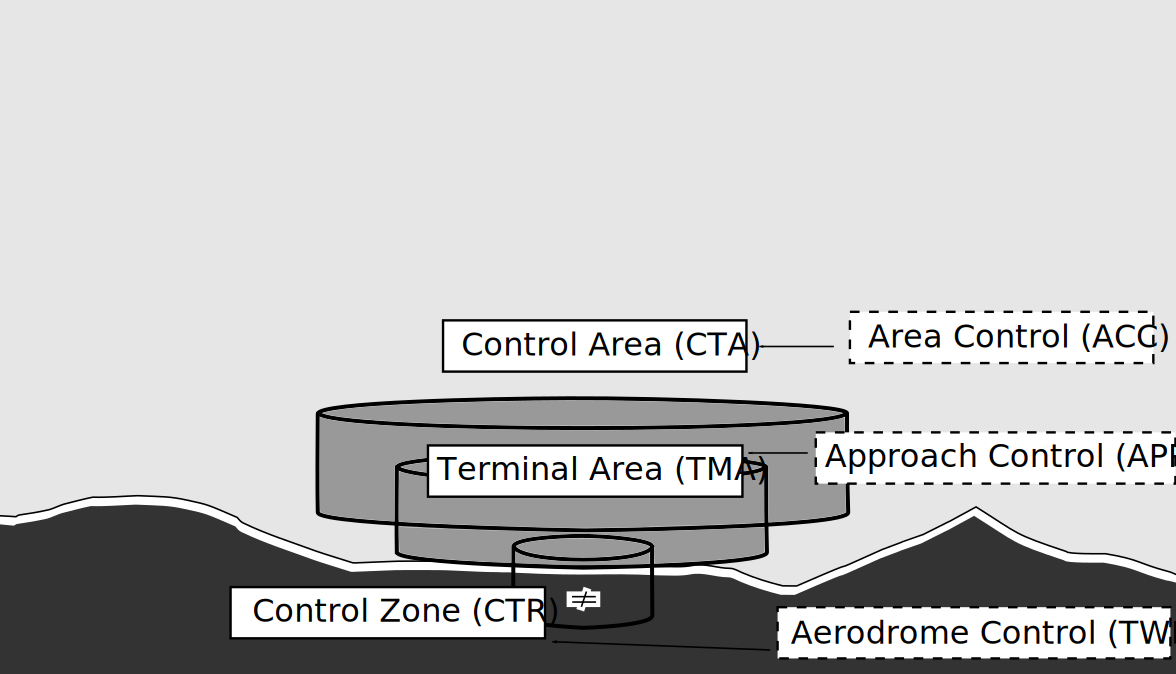
\includegraphics[width=0.8\textwidth]{figures/airspace.png}
    \caption{Airspace - \textcolor{red}{z prezentace 2011 ATM Lesson Plans/ATM 1-1 General Air Traffic Services podle \cite[Chapter 2.5]{annex11} - překreslit!}}
    \label{fig:airspace}
\end{figure}

\begin{figure}[h]
    \centering
    \includegraphics[width=0.8\textwidth]{figures/cta.png}
    \caption{CTA - \textcolor{red}{z prezentace 2011 ATM Lesson Plans/ATM 1-1 General Air Traffic Services podle \cite[Chapter 2.10]{annex11} - překreslit!}}
    \label{fig:cta}
\end{figure}

\begin{figure}[h]
    \centering
    \includegraphics[width=0.8\textwidth]{figures/airspace2.png}
    \caption{Airspace - \textcolor{red}{z prezentace 2011 ATM Lesson Plans/ATM 1-2 General Air Traffic Control Service \cite[Chapter 2.10]{annex11} - překreslit!}}
    \label{fig:airspace2}
\end{figure}

\subsubsection{Area Control Service}
Area Control Service is an ATC service provided by area control centre (ACC) responsible for flights in Control Areas (CTA). Normally ACC is identified by the name of a nearby city, area or landmark. Smaller countries usually have one ACC, but many larger countries are controlled by several of them. ACCs usually control aircrafts in their en-route phase of flight. The ACC may be also responsible for flights to and from smaller aerodromes with no separate approach control service. \cite[Chapter 3.2]{annex11}

\subsubsection{Approach Control Service}
Approach Control Service (APP) is ATC service that is responsible for the part of CTA and CTR required by arriving or departing controlled flights (TMA). The primary functions of APP is sequencing arriving aircrafts and assisting departing aircrafts becoming established on course. The arrival and departure functions can be divided into several positions on busy aerodromes. APP is usually identified by the name of the aerodrome which it is serving, but sometimes it's not colocated with TWR and is at distant ACC location. When no separate ACC exists, approach control service is provided by ACC or TWR. \cite[Chapter 3.2]{annex11}

\subsubsection{Aerodrome Control Service}
Aerodrome control service is provided by a control tower (TWR) and is responsible for aircraft landing and taking off. It's also responsible for VFR flights in the CTR and for preventing collisions between aircrafts on the manoeuvring are of the aerodrome. \cite[Chapter 3.2]{annex11}

\textcolor{red}{POKRAČOVÁNÍ: KAPITOLA 3 Z PREZENTACÍ!!!!!}

\textcolor{red}{z pohledu prostoru/z pohledu kontroly}

\textcolor{red}{v každou chvíli řídí letadlo jeden subjekt a místo a čas předání kontroly je jesně definované - kdy a jak?}

The controlled airspace can furthermore be classified as Class A-G. \cite[\textcolor{red}{kapitola}]{nolan} \textcolor{red}{popis jednotlivých classes podle nolana}

\textcolor{red}{Pro řízení v terminální oblasti nás zajímají všechny druhy řízení/prostoru, Agentfly má zatím jen ACC v CTA?}

\begin{figure}[h]
    \centering
    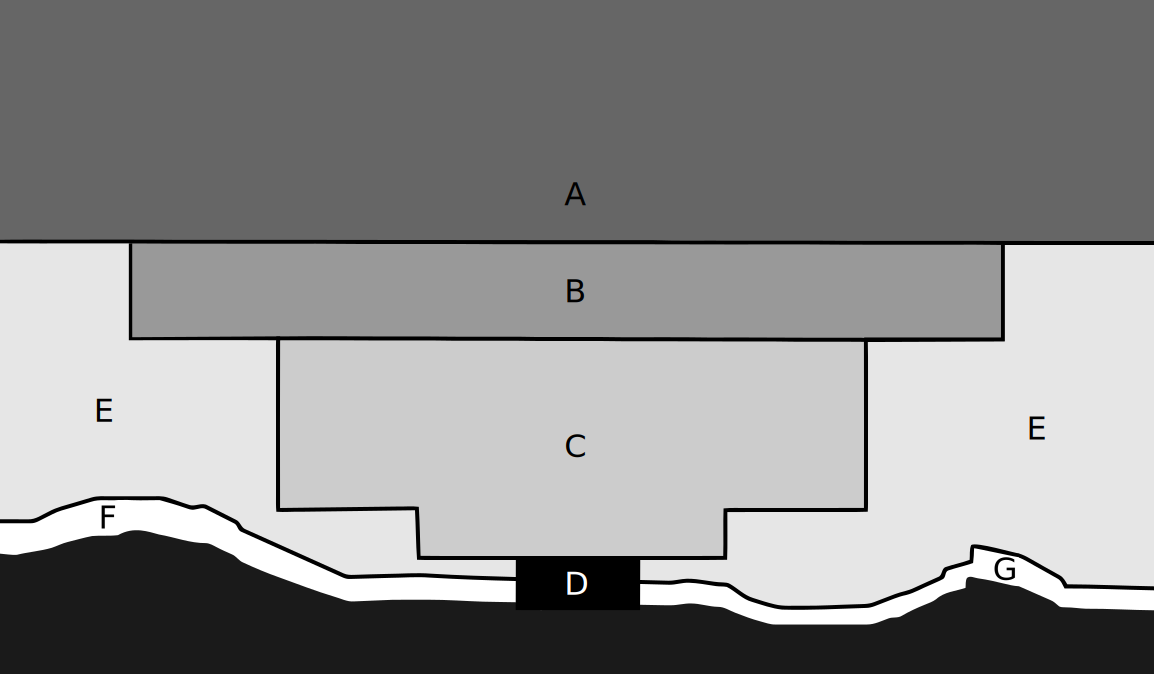
\includegraphics[width=0.8\textwidth]{figures/classes.png}
    \caption{Airspace Classification - \textcolor{red}{z prezentace 2011 ATM Lesson Plans/ATM 1-2 General Air Traffic Control Service \cite {nolan} - překreslit!}}
    \label{fig:classes}
\end{figure}

\textcolor{red}{SID a STAR routy?}